\chapter{Study 3: A Leaner Selective Pass Against a Tuned Selective-Backprop}\label{ch:study3}

This chapter answers RQ4. Study~2 showed that the selective pass saves FLOPs. Two questions remain: which design choices matter, and does the pass beat a tuned reimplementation of Selective-Backprop when every extra forward pass is charged?

\section{Exploratory search for levers}\label{sec:s3-explore}
Two exploratory rounds (\tierE{}, $10$ seeds each, seeds 2100--2109 and 2110--2119, 270 runs) varied one design choice at a time, using the literature on the closest methods (\cref{sec:related-selection}) as a source of levers: the kept fraction, the length of the full-backward warm-up, ranking rows by the norm of the last-layer gradient instead of the loss \citep{katharopoulos2018not}, a kept fraction that shrinks during training following the default rule of Ordered SGD \citep{kawaguchi2020ordered}, and a fraction that grows during training (the opposite direction, after \citealt{loshchilov2016online}). The results, with their post-hoc status, are in \cref{app:exploratory}. Two leads emerged:
\begin{enumerate}
\item A constant kept fraction of $0.15$--$0.2$ is slightly cheaper than $0.3$ (a lead of about $6$--$13\%$).
\item \textbf{Removing the warm-up} (selection from the first update on) was the largest lead. In the first round S20 without warm-up (S20w0) needed $22.7\%$ and $23.9\%$ fewer FLOPs than S30 and about half the FLOPs of A1, and was cheaper than S20 in 10 of 10 seeds. In the second round, on new seeds, the advantage over S20 shrank by about a fifth ($-13.8\%$ and $-12.0\%$ against $-17.8\%$ and $-14.6\%$), in the direction one expects from a winner's curse (the best of 14 arms was chosen), and it was cheaper in 9 and 8 of 10 seeds.
\end{enumerate}
The other levers did not help: ranking by gradient norm, the shrinking Ordered-SGD schedule, a rising fraction, a gradient rescaled by the number of kept rows, and combinations of a lower fraction with no warm-up did not pay. The warm-up dose was not graded: warm-ups of 5 and 10 steps gave about the same gain as none, and 25 steps lost most of it, a threshold-like pattern. The explanation that was tried (the second-moment estimate of the optimiser being inflated by full-size warm-up gradients) predicted a graded dose and a gain from the rescaled gradient; the first did not appear, and the second did not pass its pre-fixed bar (a scale effect of up to about $10\%$ is not excluded). \emph{No mechanism for the effect of removing the warm-up is supported by the data.} Selective-Backprop in the same rounds, run with the baseline's hyper-parameters, needed $44$--$84\%$ more FLOPs than S30 although it needed about a third fewer updates; this is the point of \cref{sec:sb-cost} below.

\section{A tuned Selective-Backprop}\label{sec:sb-cost}
A method claim needs a win against the closest published method, tuned as carefully as the proposed one. Selective-Backprop (\cref{sec:sb}) was therefore tuned once with the same 25-trial search as every other arm (learning rate, weight decay, activation, schedule; $\beta=2$, history 1\,024 and the one-epoch priming fixed in advance and not searched), on selection seeds 9200 and 9201. The winner (ReLU, cosine, learning rate $1.43\times10^{-3}$, weight decay $1.7\times10^{-6}$) needed $209.9$ GFLOPs on the two selection seeds under the uncached count of the released algorithm ($182.7$ cached), about 825 updates, at $2.28$ times the cost of a baseline step per update ($1.90$ cached). The tuned configuration is named SBT. Its cost has the structure described in \cref{sec:sb}: it needs far fewer updates, but every update is paid with an extra selection forward pass, so the FLOPs-to-target stay about level with the tuned baseline. Because $\beta$, the history length and the priming length were not searched, the result is a statement about this reimplementation with these settings.

\section{The pre-registered test (H8--H10)}\label{sec:s3-prereg}
The third pre-registration (tag \code{prereg-v3}) fixed three hypotheses for the primary arm S20w0 (kept fraction $0.2$, no warm-up), on 13 groups, 20 paired fresh seeds (2300--2319) and 260 runs, with $98.3\%$ intervals:
\begin{description}[leftmargin=2.6em,style=nextline]
\item[H8] S20w0 needs at least $15\%$ fewer FLOPs-to-target than the tuned baseline A1, with the re-tuning shift of \cref{sec:stats}.
\item[H9] S20w0 needs at least $10\%$ fewer FLOPs than S30 (the variant of Study~2), no shift.
\item[H10] S20w0 needs at least $15\%$ fewer FLOPs than the tuned Selective-Backprop SBT, no shift, \emph{uncached count decisive} and the cached count reported next to it.
\end{description}
H9 is the least independent of the three, because S20w0 differs from S30 in two choices (fraction and warm-up); it is kept so that the S30 reference of Study~2 is not skipped, and the split is reported below. No batch-size control is repeated, because S20w0 changes neither the batch size nor the optimiser, and S itself is not tuned again. The five re-tunings of the baseline A2, A5--A8 were re-run on the new seeds for the shift; the descriptive groups S20, S15, S20w10 and the random control R20w0 complete the design. Every one of the 260 runs was started at the lock commit with a clean working tree.

\section{Results}\label{sec:s3-results}
\begin{table}[t]
\centering\small
\caption{Study 3: mean GFLOPs-to-target, mean steps (optimizer updates) among the runs that reached the target, runs that never reached it, and paired change against A1 ($98.3\%$ bootstrap intervals), 20 seeds per group. For SBT the FLOPs are the uncached count. The re-tunings A2, A5--A8 define the shift.}
\label{tab:s3-main}
\resizebox{\textwidth}{!}{%
\begin{tabular}{@{}l rrr l rrr l@{}}
\toprule
 & \multicolumn{4}{c}{target 0.97} & \multicolumn{4}{c}{target 0.975}\\
\cmidrule(lr){2-5}\cmidrule(l){6-9}
Group & GFLOPs & steps & never & change (\%) & GFLOPs & steps & never & change (\%)\\
\midrule
A1 (tuned baseline) & 145.8 & 940 & 0 & -- & 222.5 & 1435 & 0 & -- \\
A2 & 193.0 & 1245 & 0 & $+32.4$ [$+22.9$, $+42.4$] & 247.7 & 1598 & 0 & $+11.3$ [$+4.9$, $+18.7$] \\
A5 & 142.7 & 920 & 0 & $-2.1$ [$-10.4$, $+8.0$] & 213.6 & 1378 & 0 & $-4.0$ [$-11.3$, $+3.7$] \\
A6 & 150.4 & 970 & 0 & $+3.2$ [$-4.7$, $+11.9$] & 219.4 & 1415 & 0 & $-1.4$ [$-7.0$, $+5.1$] \\
A7 & 145.4 & 938 & 0 & $-0.3$ [$-8.1$, $+8.2$] & 216.3 & 1395 & 0 & $-2.8$ [$-11.9$, $+5.5$] \\
A8 & 153.9 & 992 & 0 & $+5.6$ [$-2.6$, $+14.1$] & 222.1 & 1432 & 0 & $-0.2$ [$-6.9$, $+7.8$] \\
\midrule
SBT (Selective-Backprop, tuned) & 140.3 & 632 & 0 & $-3.7$ [$-12.9$, $+6.6$] & 245.4 & 922 & 0 & $+10.3$ [$+1.6$, $+19.7$] \\
\midrule
S30 & 96.6 & 952 & 0 & $-33.7$ [$-38.3$, $-28.5$] & 140.8 & 1418 & 0 & $-36.7$ [$-39.7$, $-34.0$] \\
S20 & 89.5 & 958 & 0 & $-38.6$ [$-42.9$, $-33.8$] & 128.2 & 1405 & 0 & $-42.4$ [$-45.1$, $-39.9$] \\
S15 & 85.7 & 952 & 0 & $-41.2$ [$-45.4$, $-36.5$] & 122.7 & 1402 & 0 & $-44.9$ [$-47.6$, $-41.8$] \\
S20w10 & 77.1 & 885 & 0 & $-47.1$ [$-51.6$, $-41.6$] & 111.2 & 1280 & 0 & $-50.0$ [$-54.5$, $-46.1$] \\
S20w0 (primary arm) & 75.1 & 870 & 0 & $-48.5$ [$-52.1$, $-44.2$] & 114.0 & 1320 & 0 & $-48.8$ [$-53.4$, $-43.8$] \\
\midrule
R20w0 (random 20\%, no warm-up) & 192.7 & 2232 & 0 & $+32.2$ [$+23.3$, $+42.5$] & 256.8 & 2833 & 17 & $+15.4$ [$+7.6$, $+23.4$]
\\
\bottomrule
\end{tabular}}
\end{table}

\begin{keyfinding}
\textbf{H8, H9 and H10 are all supported.} S20w0 needed $48.5\%$ ($[-52.1,-44.2]$) and $48.8\%$ ($[-53.4,-43.8]$) fewer FLOPs than the tuned baseline, $22.2\%$ ($[-29.1,-14.7]$) and $19.1\%$ ($[-26.1,-11.7]$) fewer than S30, and $46.5\%$ ($[-52.3,-40.3]$) and $53.6\%$ ($[-58.3,-48.2]$) fewer than the tuned Selective-Backprop (uncached count), at $0.97$ and $0.975$. The largest gain of any re-tuning of A1 was $2.1\%$ and $4.0\%$, far below $48\%$. S20w0 was cheaper than A1 and than SBT in 20 of 20 seeds at both targets, and cheaper than S30 in 19 and 18 of 20.
\end{keyfinding}

\begin{figure}[t]
\centering
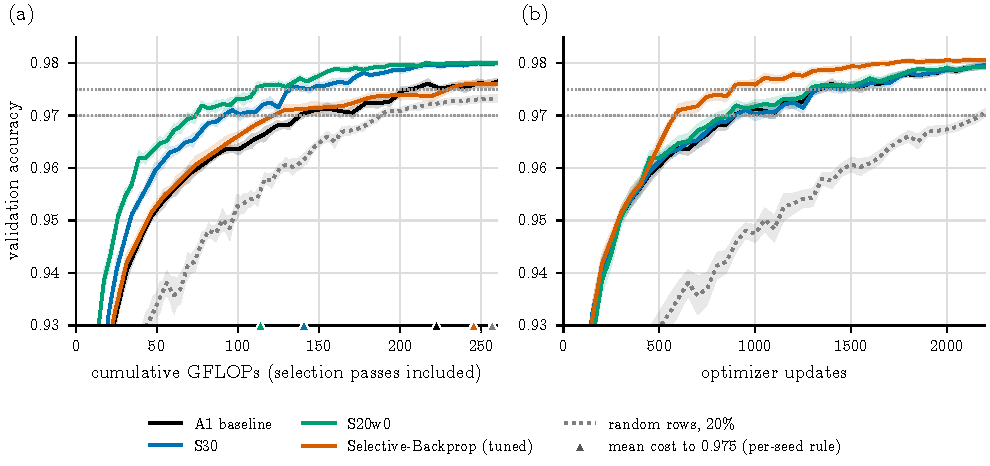
\includegraphics[width=\textwidth]{fig_s3_curves}
\caption{Study 3 (20 seeds, $95\%$ bands). (a) Validation accuracy against cumulative GFLOPs, with all selection passes charged. (b) The same runs against the number of optimiser updates. In updates, S20w0 is only slightly ahead of the baseline and Selective-Backprop is far ahead; in FLOPs the order is reversed.}
\label{fig:s3-curves}
\end{figure}

\begin{figure}[t]
\centering
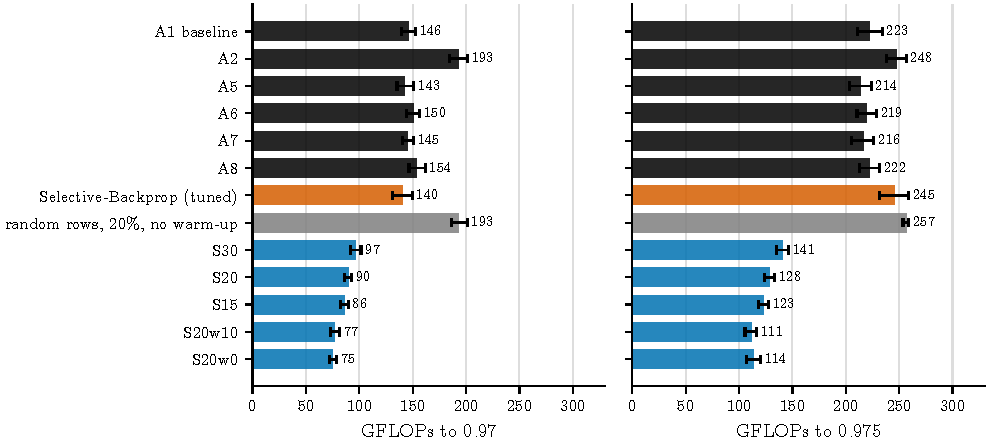
\includegraphics[width=\textwidth]{fig_s3_bars}
\caption{Mean GFLOPs to reach $0.97$ (left) and $0.975$ (right) for all 13 groups of Study 3, with $95\%$ bootstrap intervals of the mean (black: baseline tunings; orange: Selective-Backprop; grey: random rows; blue: selective variants). The six baseline tunings are close to each other on these seeds; every selective variant with top-$k$ selection is far below them.}
\label{fig:s3-bars}
\end{figure}

\begin{figure}[t]
\centering
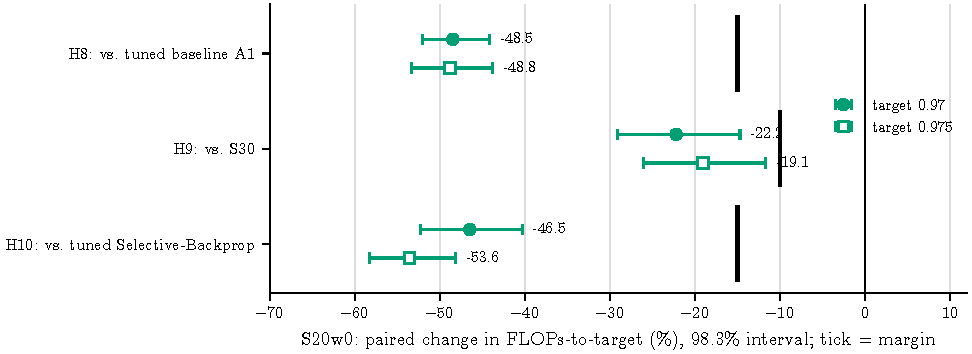
\includegraphics[width=0.82\textwidth]{fig_s3_forest}
\caption{The three pre-registered comparisons of Study 3 ($98.3\%$ intervals). The black tick on each row is the margin fixed in advance. All intervals are far beyond their margins.}
\label{fig:s3-forest}
\end{figure}

\begin{figure}[t]
\centering
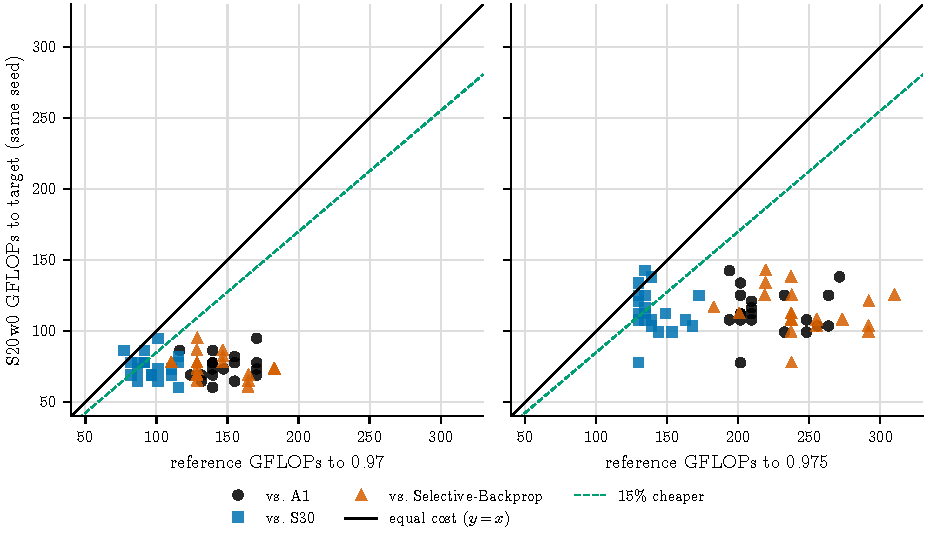
\includegraphics[width=0.95\textwidth]{fig_s3_paired}
\caption{Seed-by-seed comparison. Each point is one seed: the cost of S20w0 against the cost of a reference on the same seed, at target $0.97$ (left) and $0.975$ (right). Points below the black diagonal favour S20w0; the dashed green line is a $15\%$ saving. Against the baseline and against Selective-Backprop every point is below the $15\%$ line; against S30 most are, but not all.}
\label{fig:s3-paired}
\end{figure}

\paragraph{Why Selective-Backprop loses in FLOPs.} The curves of \cref{fig:s3-curves}b show Selective-Backprop in updates: it needs only $632$ and $922$ updates to reach the two targets against $940$ and $1435$ for A1. If the cost of a method were its step count it would be the best of all. But each update of the released algorithm is paid with selection forward passes over batches that are mostly discarded and a second forward pass over the kept rows ($2.28$ times the cost of a baseline step in the tuned run). Its FLOPs-to-target are $-3.7\%$ ($[-12.9,+6.6]$) and $+10.3\%$ ($[+1.6,+19.7]$) relative to A1: level with the baseline. Even an implementation that reuses the selection pass (the cached count) reaches the targets with $13.3\%$ and $5.0\%$ fewer FLOPs than A1 (the second is not distinguishable from zero), and S20w0 is still $40.5\%$ and $46.1\%$ cheaper than that (\cref{tab:s3-secondary}). The selective pass of this report keeps the top rows of a batch it has \emph{already} run forward, so it pays no additional selection pass. This is the source of its advantage in FLOPs, not a better selection rule.

\paragraph{Secondary readings.} \Cref{tab:s3-secondary} lists the readings that decide nothing.
\begin{table}[t]
\centering\small
\caption{Study 3, secondary readings (descriptive; $98.3\%$ intervals).}
\label{tab:s3-secondary}
\begin{tabular}{@{}l l l@{}}
\toprule
Reading & to 0.97 & to 0.975\\
\midrule
S20w0 vs.\ SBT, cached count (FLOPs) & $-40.5$ $[-46.6,-34.1]$ & $-46.1$ $[-51.4,-40.1]$\\
SBT vs.\ A1, uncached / cached (FLOPs) & $-3.7$ / $-13.3$ & $+10.3$ / $-5.0$\\
S20w0 vs.\ S20 (FLOPs) & $-16.1$ $[-21.9,-10.0]$ & $-11.1$ $[-18.5,-3.3]$\\
S20w0 vs.\ S20 (steps) & $-9.1$ $[-15.6,-2.4]$ & $-6.0$ $[-14.0,+2.3]$\\
S20w0 vs.\ S20w10 (FLOPs) & $-2.6$ $[-10.3,+5.8]$ & $+2.5$ $[-5.5,+10.6]$\\
S20w0 vs.\ S15 (FLOPs) & $-12.3$ $[-20.0,-4.2]$ & $-7.1$ $[-15.6,+0.9]$\\
S20w0 vs.\ random rows R20w0 (FLOPs) & $-61.0$ $[-64.5,-57.5]$ & $-55.6$ $[-59.0,-52.2]$\\
\bottomrule
\end{tabular}
\end{table}

\paragraph{Where the saving comes from.} \Cref{fig:waterfall} decomposes the saving against A1 at target $0.975$. Moving from the full backward pass to S30 saves $81.7$ GFLOPs, a lower kept fraction ($0.3\to0.2$) a further $12.6$, and removing the warm-up another $14.2$. About $6.9$ of these $14.2$ GFLOPs is pure arithmetic: the 100 warm-up steps of S20 were charged as full steps, and are charged as selective steps in S20w0. The rest, $7.3$, comes from reaching the target in fewer steps (S20w0 needed $6$--$9\%$ fewer steps than S20, though the interval at $0.975$ includes zero). A warm-up of only 10 steps (S20w10) is level with no warm-up at all (FLOPs $-2.6\%$ and $+2.5\%$ with intervals around zero), so the benefit of dropping the warm-up is not specific to the exact value zero.

\begin{figure}[t]
\centering
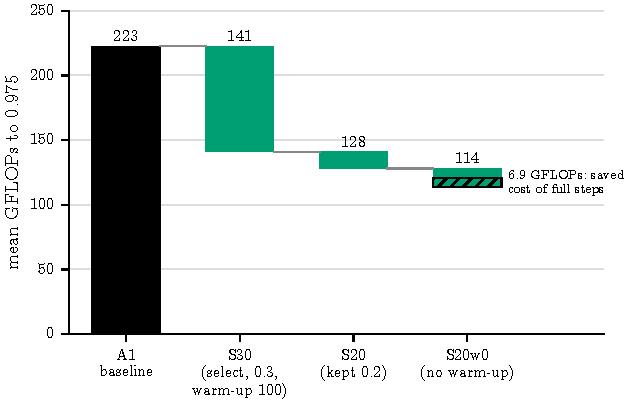
\includegraphics[width=0.62\textwidth]{fig_s3_waterfall}
\caption{Decomposition of the saving against the baseline (mean GFLOPs to $0.975$, 20 seeds of Study~3). Hatched: the part of the last step that is the saved arithmetic cost of the 100 warm-up steps.}
\label{fig:waterfall}
\end{figure}

\paragraph{Random rows.} Keeping 20\% of the rows at random without warm-up (R20w0) needs $+32.2\%$ and $+15.4\%$ more FLOPs than A1, fails to reach $0.975$ in 17 of 20 seeds, and S20w0 is $61\%$ and $56\%$ cheaper than R20w0 on the same seeds (R20w0 costs about $2.6$ and $2.3$ times as much). The ranking of rows by loss is what keeps the number of steps low, and removing the warm-up is harmless only when the rows kept are the informative ones.

\section{Interpretation and limits}
\begin{itemize}
\item The pre-registered claim is a statement about \emph{FLOPs-to-target in this setting}, with every selection pass charged. It does not say that S20w0 is faster than Selective-Backprop in time: Selective-Backprop's published gains are measured in wall-clock time on deep image models, which this study does not reproduce, and the report's per-step timing of S30 shows that the FLOPs saving of the selective pass is much larger than its time saving (\cref{sec:wallclock}). S20w0 itself was not timed.
\item SBT was tuned once with three of its design parameters fixed in advance, and its selection score is in-sample, like that of any arm. The reading that it is level with the baseline in FLOPs depends on these choices.
\item H9 combines two changes (fraction and warm-up); the split (S20 against S30, S20w0 against S20) is exploratory.
\item There is no supported mechanism for why removing the warm-up helps. An obvious guess (that the full-size warm-up gradients inflate the optimiser's second-moment estimate and slow the later, smaller selective gradients) predicted a graded dose-response and a benefit of rescaling the gradient; the dose was not graded and the rescaling did not pass its bar.
\item The result was generated by selecting the best of a set of exploratory arms and then replicated on fresh seeds; the confirmatory test is on new seeds, so the winner's curse of the exploratory rounds does not affect the verdicts. The size of the effect in the confirmatory test ($-48.5\%$ against A1) is close to the exploratory pooled estimate ($-49\%$ to $-51\%$), and the advantage over S30 ($-22.2\%$ and $-19.1\%$) is also consistent with the first round ($-22.7\%$ and $-23.9\%$).
\end{itemize}

\section{Summary of Study 3}
A lean variant of the selective backward pass (keep $20\%$ of the rows, no full-backward warm-up) beat the tuned baseline, the first selective variant and a tuned Selective-Backprop reimplementation in FLOPs-to-target, in a pre-registered test on 20 fresh seeds, by margins far above those fixed in advance. The advantage over Selective-Backprop comes from not paying for extra selection passes. Everything is conditional on this network and on counted FLOPs.
